
\section{Präsentation und Auswertung der Ergebnisse} \label{sec:Erg}
Für die Darstellung der Ergebnisse des Projekts soll zunächst der entwickelte Algorithmus zur Berechnung des Stromverbrauchs im optimierten Netz beschrieben werden. Anschließend wird in Kapitel \ref{subsec:ErgSoftware} ausführlich auf die erstellte Software \textquote{EnergyNetSim} und deren Benutzung eingegangen, bevor in Kapitel \ref{subsec:ErgDiskussion} eine Diskussion der Ergebnisse und Erkenntnisse folgt.

\subsection{Algorithmus zum dynamischen Routing der Netzlast-Ströme} \label{subsec:ErgAlg}
Wie in Kapitel \ref{subsec:VorgAlg} dargestellt, wurde ein Algorithmus entwickelt, der es erlaubt, Netzlast (Traffic) dynamisch durch ein definiertes Netz zu routen und anschließend nicht benötigte Geräte und Verbindungen abzuschalten.
Grundlegend ist das Ziel, für jeden Zeitabschnitt die beste erzielbare Lösung zur stromsparenden Bewältigung (Durchleitung) des Traffics von dem Eingangspunkt in das Netz (Quelle) bis zum Austrittspunkt (Senke) zu berechnen. Zur Vereinfachung wurde die Annahme getroffen, dass über die Dauer eines Zeitabschnittes (einer Iteration) die durch den Algorithmus getroffenen Routing-Entscheidungen und die Wahl der abzuschaltenden Hardware gleich bleiben. Geht man von 24 Iterationen aus, so würde also der Zustand des Netzes für jede Stunde neu berechnet werden. Durch eine Verkürzung der Iterationsdauer und Generierung dazu passender Netzlast-Daten ließe sich bei Bedarf mit geringem Aufwand ein genaueres, verfeinertes Modell durchrechnen, so dass ein realistischeres Resultat zu erwarten ist.


\begin{figure}[!ht]
	\centering
	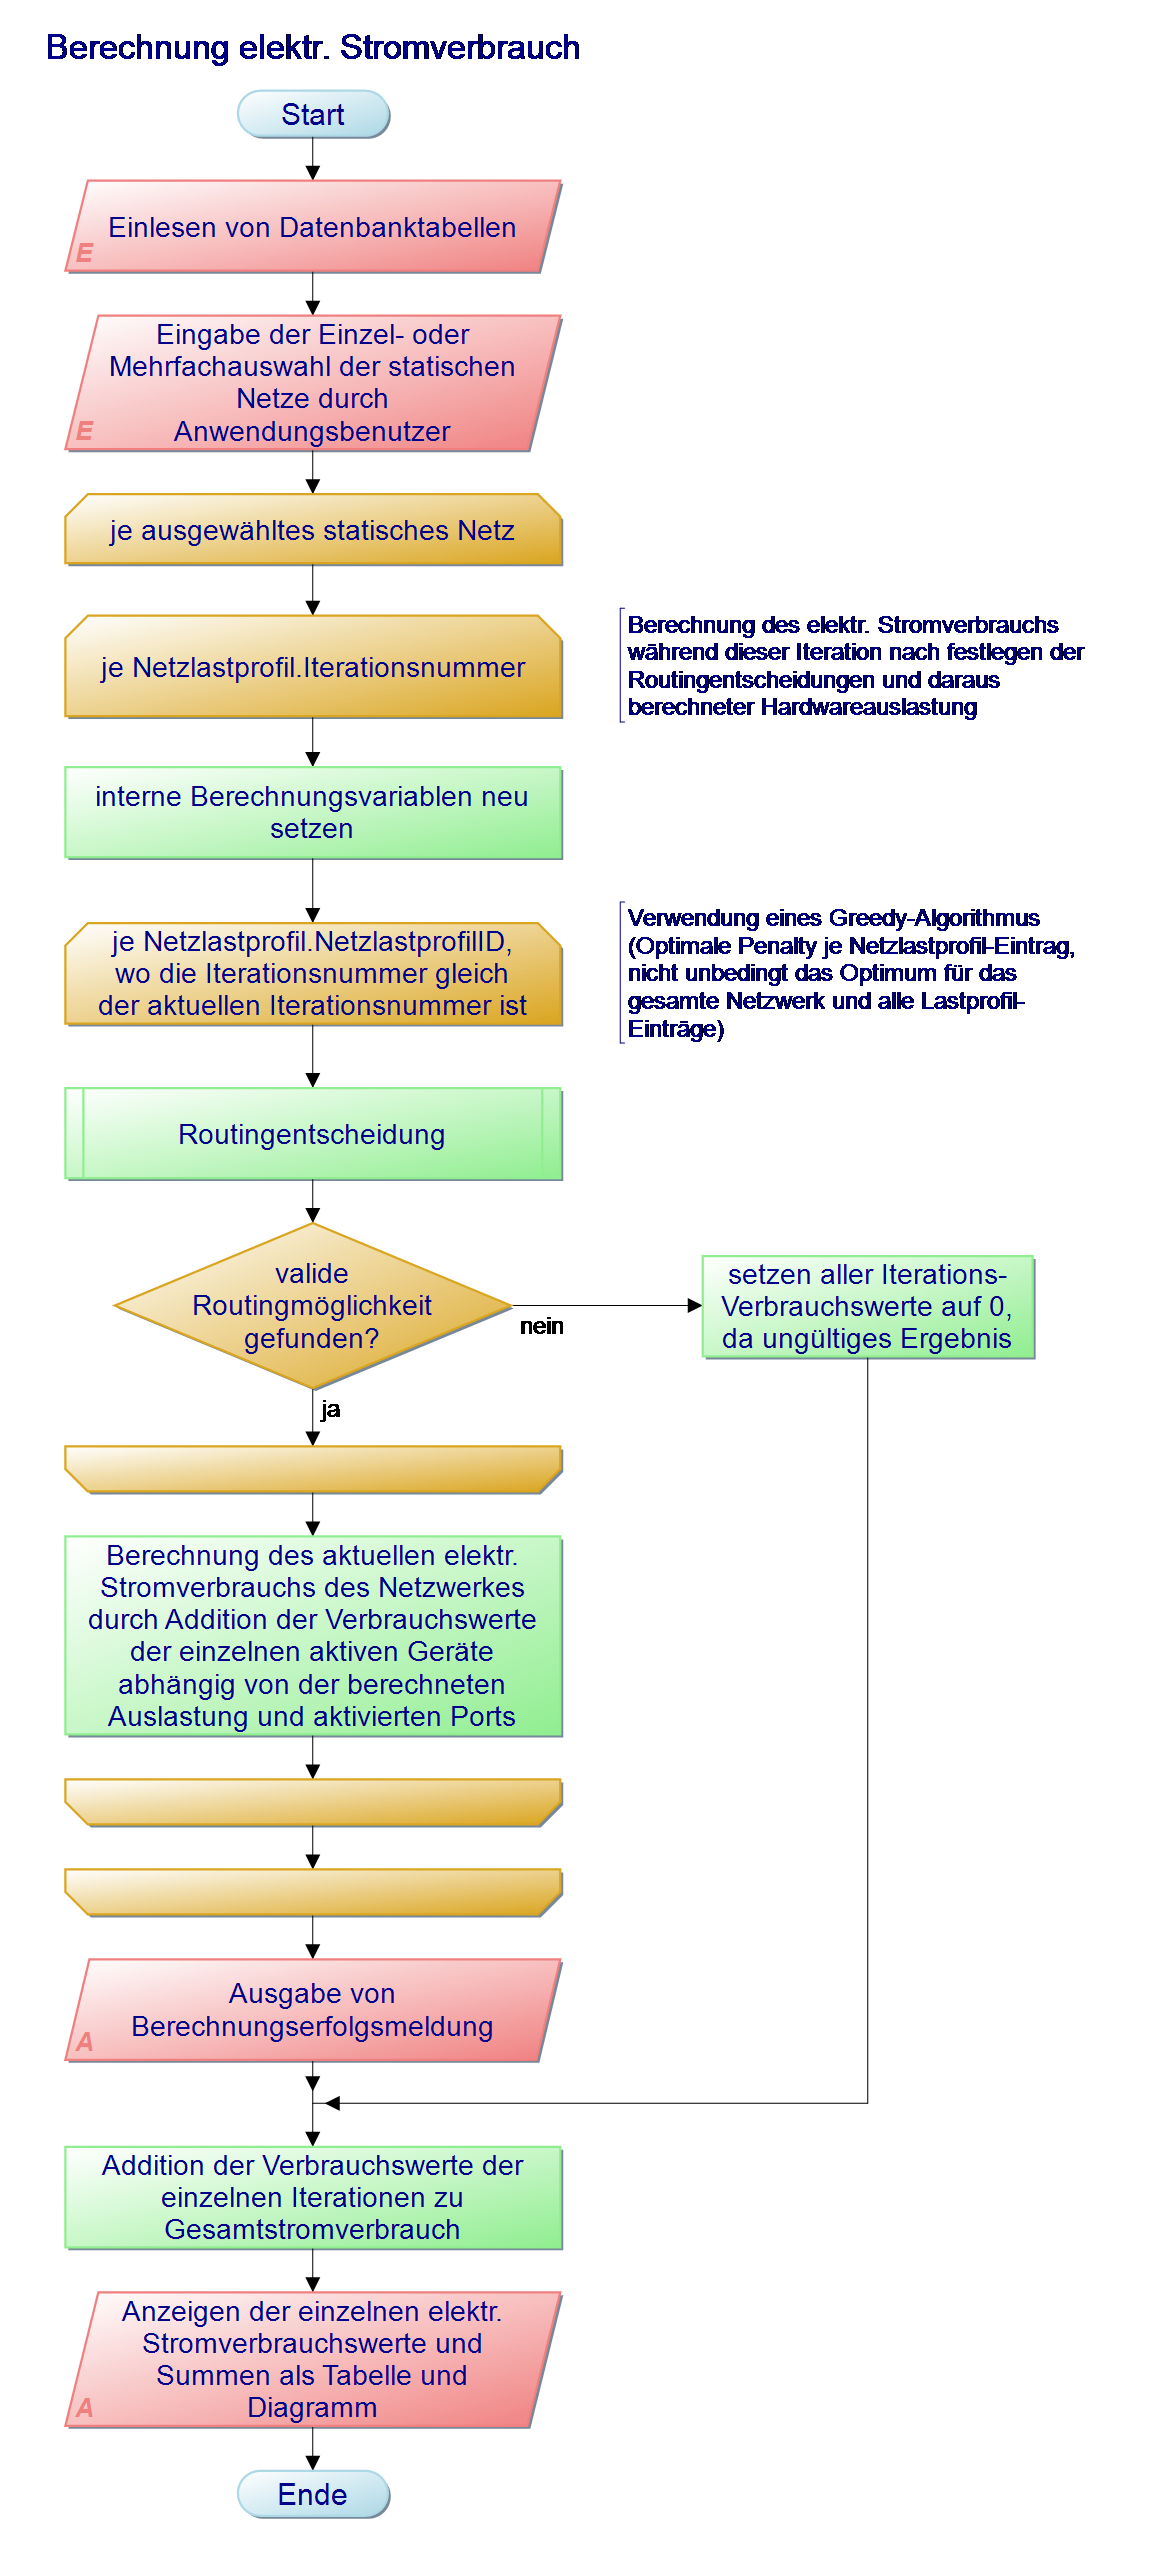
\includegraphics[width=0.6\textwidth]{1Berechnung_elektr_Stromverbrauch}
	\caption{Programmablaufplan zur Anwendungslogik}
	\label{fig:1Berechnung_elektr_Stromverbrauch}
\end{figure}


Für jedes zu vergleichende Netz wird eine Datenreihe bestehend aus einem Stromverbrauchswert je Iterationszeitraum berechnet. Um die Einzelwerte zu berechnen, werden zuerst die Lasten aus jedem Netzlastprofil-Eintrag möglichst effizient auf die Netzwerkhardware und Verbindungen projiziert, und danach abschließend abhängig von den berechneten Geräteauslastungen die Teil-Stromverbrauchswerte addiert.


Mit der geschilderten Vorgehensweise lässt sich das gesuchte Ergebnis je Modellnetzwerk inklusive des zeitlichen Verlaufs errechnen. Allerdings fehlt dazu noch die Antwort auf die Frage, wie die effizienten Routing-Entscheidungen getroffen werden können. Der folgende Teil des Algorithmus beschreibt eine mögliche Lösung:


Um zu entscheiden, welches Routing für die einzelnen Netzlastprofil-Einträge je Iteration das beste Resultat liefert, wird je möglicher Route eine dynamische Penalty (Kosten-Faktor) berechnet. Anschließend wird für das Netzlastprofil die Route mit der niedrigsten errechneten Penalty, welche die Datendurchsatzgrenzen der Hardware und somit der einzelnen Verbindungen nicht überschreiten, als beste Route angenommen. Es handelt sich um einen sogenannten Greedy Algorithmus, ein lokales Lösungsverfahren, das nicht unbedingt das insgesamt beste Ergebnis liefert. Vielmehr wird nur das lokale Optimum für das betrachtete Teilproblem, hier also das Routing für ein Netzlast-Element, berechnet. Um eine schnelle praktische Ausführungszeit auch bei Berechnungen mehrerer Vergleichsnetze mit kurzen Iterationsintervallen zu erreichen, beinhaltet der entwickelte Algorithmus intelligente Entscheidungsfunktionen.  So werden schlechte Routen frühzeitig ignoriert und nicht zielführende Berechnungen, wie sie beispielsweise bei Schleifenbildung auftreten, verhindert.
\begin{figure}[ht]
	\centering
	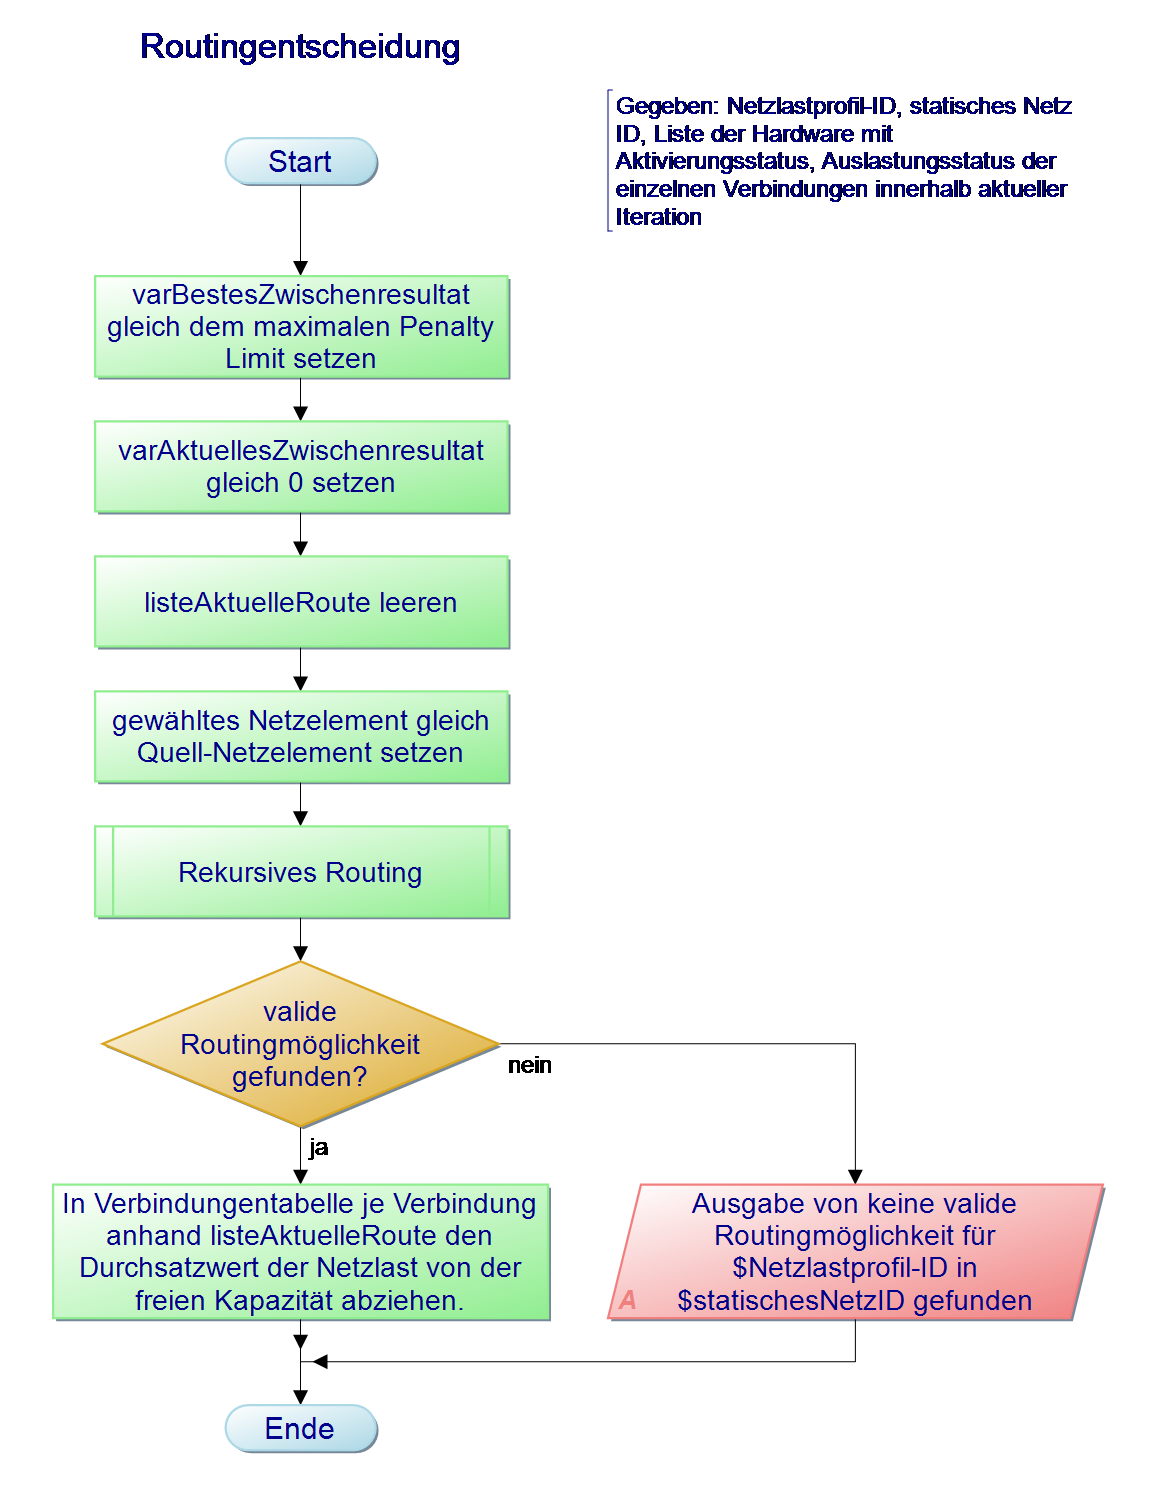
\includegraphics[width=0.6\textwidth]{2Routingentscheidung}
	\caption{Programmablaufplan zum übergreifenden Anteil des Routing-Algorithmus}
	\label{fig:2Routingentscheidung}
\end{figure}

Da die zur Verbindungsbewertung verwendete Penalty mehreren Faktoren wie Latenz, elektrischer Stromverbrauch, Kapazität der Verbindung und auch An-/Aus-Status der Hardware berücksichtigen muss, und die genannten Faktoren je nach Verwendungszweck des Netzes unterschiedliche Gewichtung haben, müssen die einzelnen Anteile mit vom Anwender der Simulationssoftware festgelegten Gewichtungsfaktoren multipliziert werden. Damit kann der Nutzer die Netzsimulation auf seine Anforderungen ansatzweise anpassen.
\begin{figure}[ht]
	\centering
	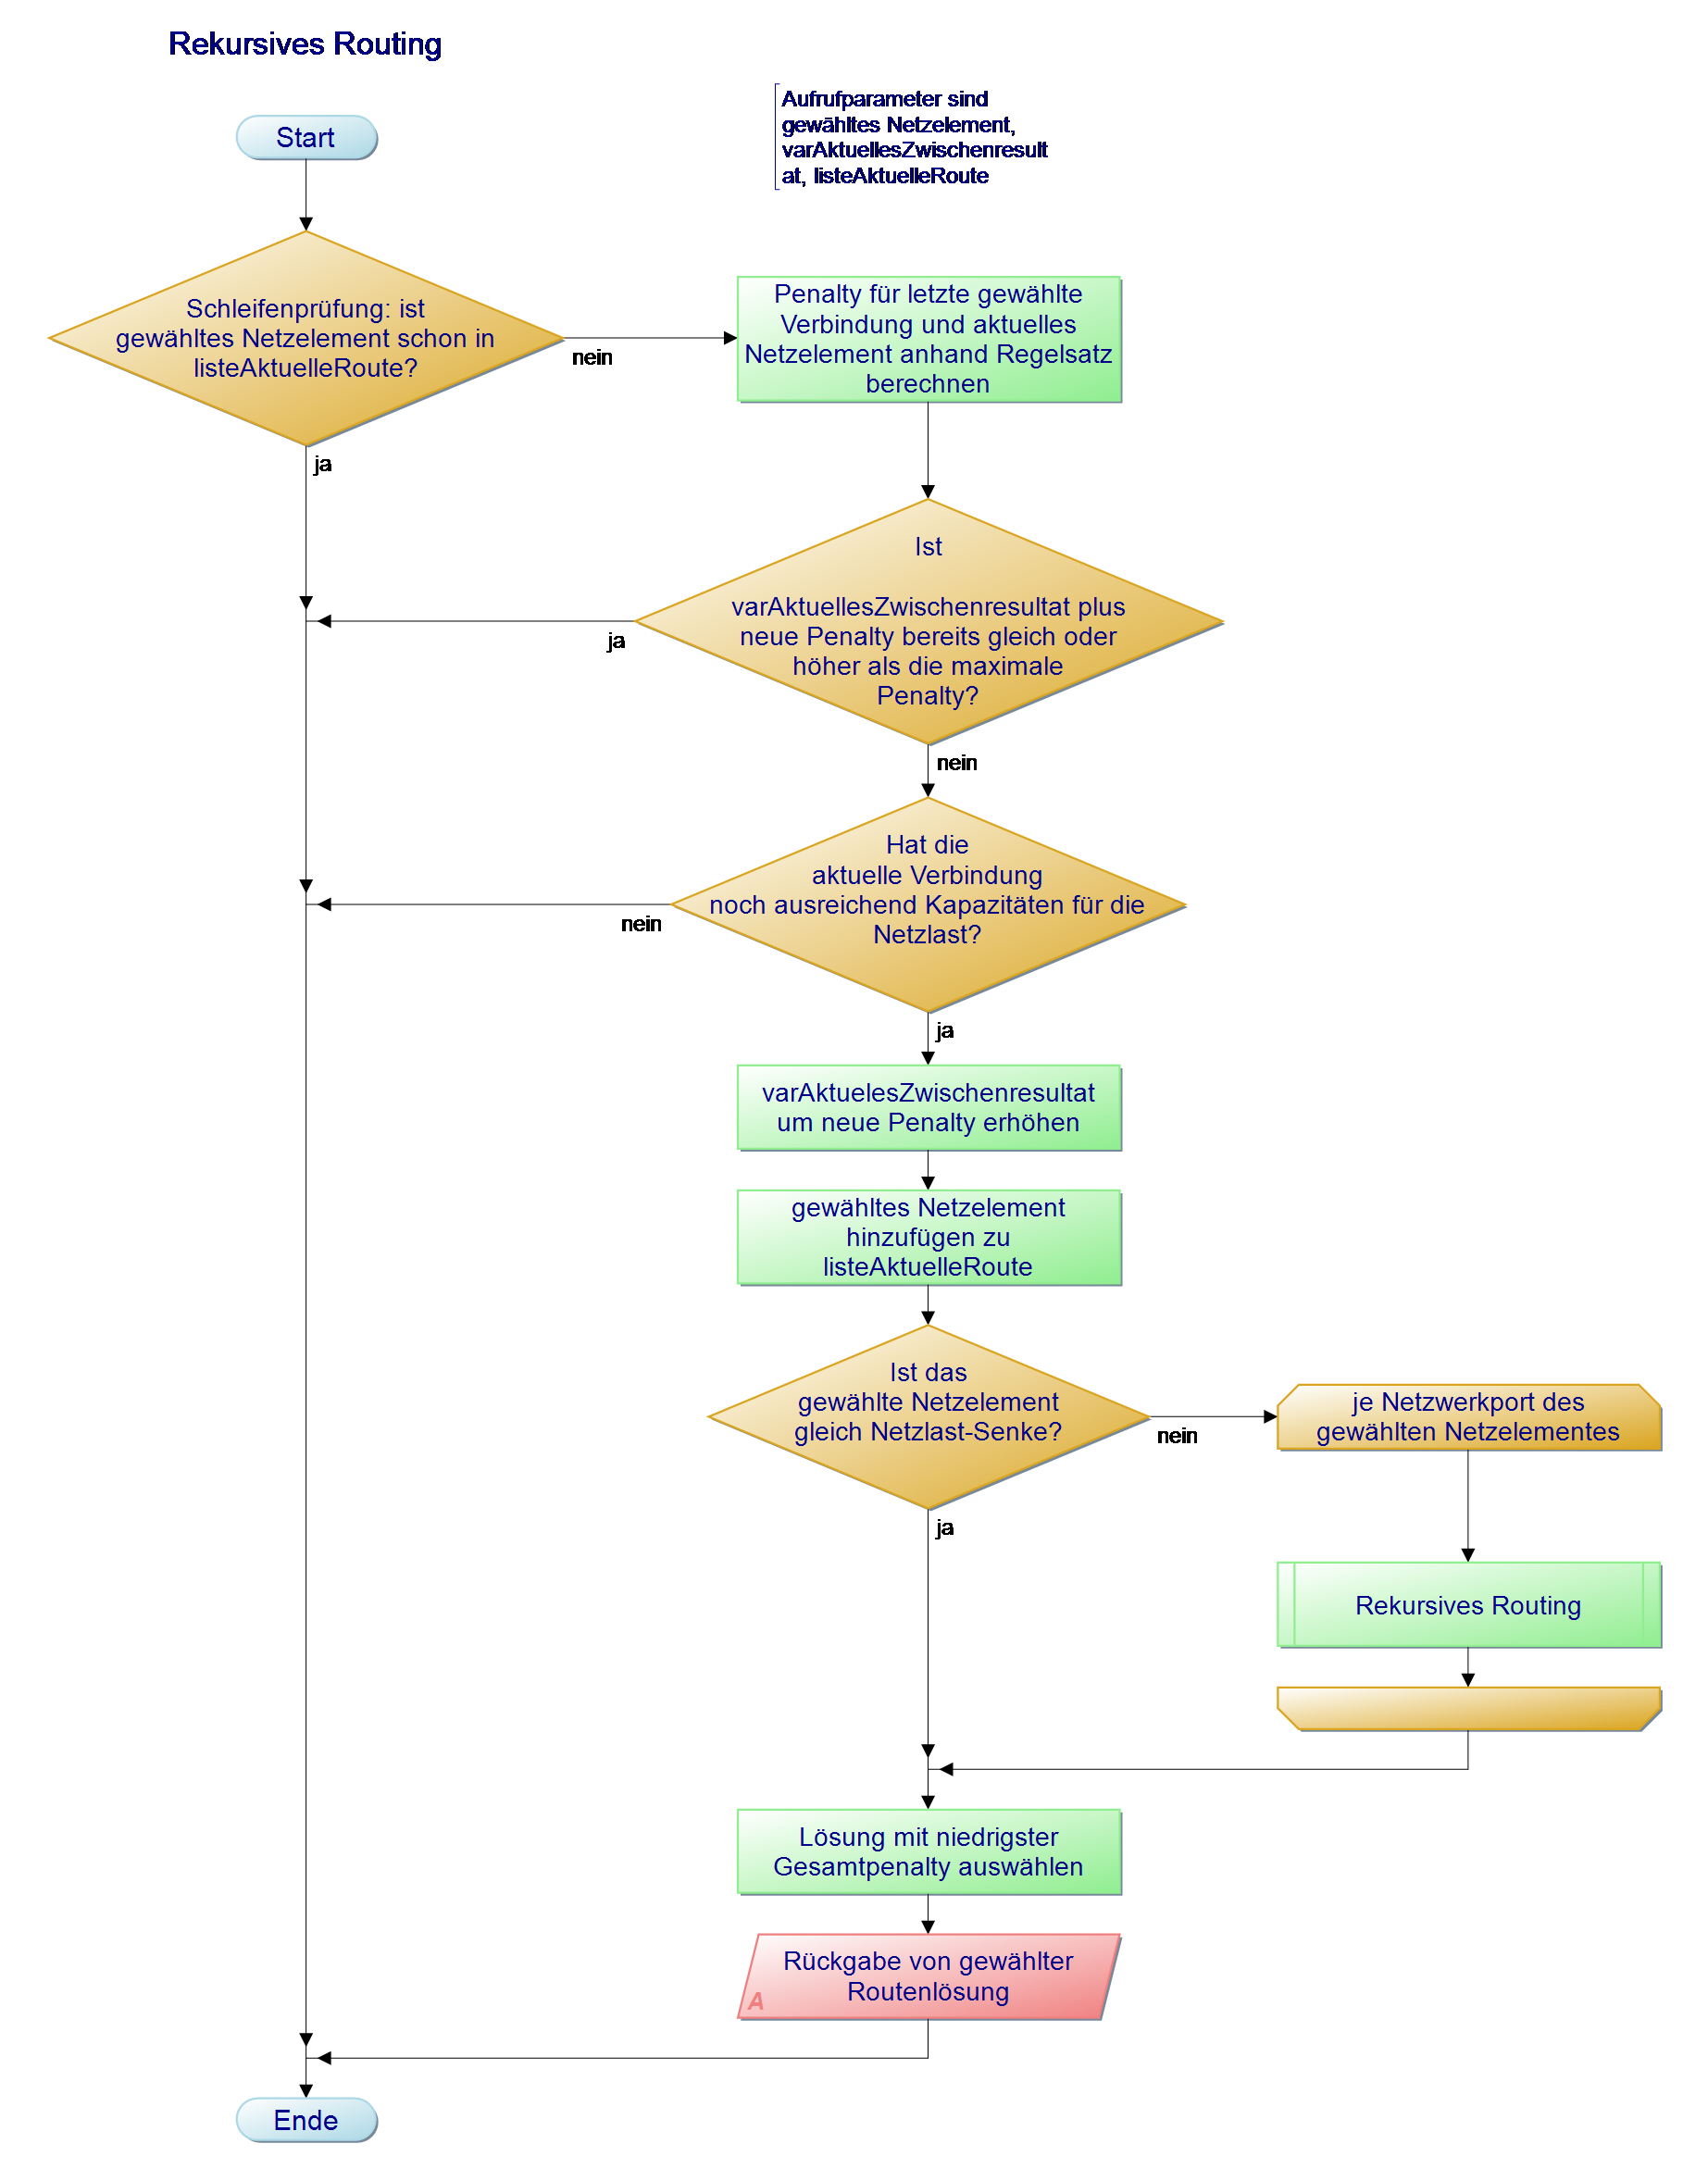
\includegraphics[width=0.6\textwidth]{3Rekursives_Routing}
	\caption{Rekursiver Anteil des Routing-Algorithmus}
	\label{fig:3Rekursives_Routing}
\end{figure}


Alles in allem ist ein Regelsatz zur Penaltyberechnung je Iteration notwendig, an Hand dessen die Algorithmus-Implementierung jeweils versucht, das lokale Optimum zum Routingproblem als Lösung zu finden.
Der folgende Regelsatz ergab sich aus dem Durchlaufen einer solchen Simulation auf dem Papier:
\begin{itemize}
	\item Zum Anfang jeder neuen Iterations-Zeitphase sind alle Geräte und alle Ports (sofern sie dazu in der Lage sind) ausgeschaltet
	\item Das Aktivieren eines Devices kostet Penalty (hoch)
	\item Das Aktivieren eines Ports kostet Penalty (niedrig)
	\item Das Ausschalten des Port-Energiesparmodus kostet keine Penalty, um vermeidbares aktivieren anderer Hardware / Ports zu vermeiden. Energiesparmodus-Capability zählt lediglich zur Berechnung des Stromverbrauchs.
	\item Um niedrige Paketlaufzeiten durch das Netz sicherzustellen, kostet jeder Hop / genutzte Verbindung eine weitere Penalty (hoch)
\end{itemize}
Einzelne Verbindungen haben zusätzlich zu dem dynamischen Anteil außerdem jeweils eine feste Penalty, die sich aus  ihrer Länge und damit der Anzahl an Signalverstärkern ergibt und statisch in der Datenbank hinterlegt ist.

\subsection{Die erstellte Software aus Ergebnissicht}\label{subsec:ErgSoftware}
Im Rahmen der Software-Entwicklung wurde das Java-Programm \textquote{EnergyNetSim} mitsamt Anbindung an eine MySQL-Datenbank realisiert. Die folgenden Unterkapitel beschreiben die erzielten Resultate und geben Hinweise auf Installation und Benutzung der Software für Endanwender.

\subsubsection{Ergebnisse der Software-Entwicklung}
Die erstellte Software \textquote{EnergyNetSim} stellt ein Rahmenwerk zur Verfügung, in das die in den Kapiteln
\ref{subsec:VorgAlg} und \ref{subsec:ErgAlg} beschriebenen Algorithmen zur Simulation von Netzauslastung, Datenverkehr zwischen zwei Netzknoten, dynamischem Routing und effizienzsteigernden Energiesparmechanismen eingefügt werden können. Im Programmcode und in der Dokumentation sind die dazu notwendigen Methoden bereits angelegt und gekennzeichnet. Das Kapitel \ref{subsubsec:ErgSoftwErweiterung} gibt dazu detailliertere Hinweise.
Aufgaben wie die Selektion der zu betrachtenden Netze, die einfache Adaption von Parametern zur Simulation, die persistente Speicherung der Konfigurationen und Netzstrukturen und die graphische Ausgabe der errechneten Ergebnisse übernimmt der aktuelle Softwarestand bereits. Die Grundlage dafür bietet die Einbindung der frei verfügbaren Java-Bibliothek \textquote{jFreeChart}\footnote{\textquote{JFreeChart is a free 100\% Java chart library that makes it easy for developers to display professional quality charts in their applications. JFreeChart's extensive feature set includes, a consistent and well-documented API, supporting a wide range of chart types; a flexible design that is easy to extend,[…] support for many output types, including Swing and JavaFX components, image files (including PNG and JPEG).[…] JFreeChart is open source or, more specifically, free software. It is distributed under the terms of the GNU Lesser General Public Licence (LGPL), which permits use in proprietary applications.} \cite{jdbc}} und des offiziellen JDBC-Treibers\footnote{Frei verfügbar unter https://dev.mysql.com/downloads/connector/j/5.1.html} zur Verbindung mit der MySQL-Datenbank.
\begin{figure}[ht]
	\centering
	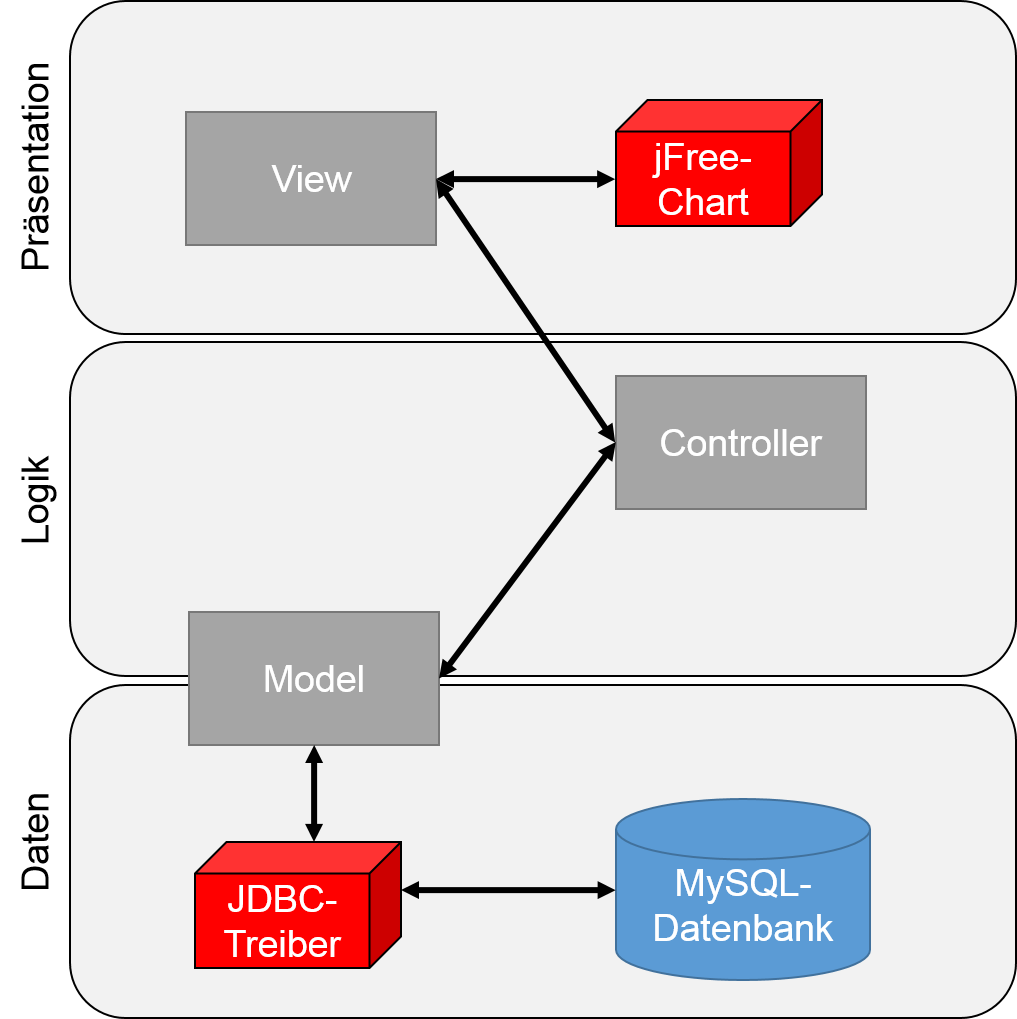
\includegraphics[width=0.5\textwidth]{ErgSoftwareMVC}
	\caption{Schichtenarchitektur des EnergyNetSim (eigene Darstellung)}
	\label{fig:ErgSoftwareMVC}
\end{figure}
Das Zusammenspiel zwischen Java-Anwendung und der MySQL-Datenbank zeigt
Abbildung \ref{fig:ErgSoftwareMVC}. Bei der Entwicklung wurde ein \textquote{Model-View-Controller} (kurz: MVC)-Entwurfsmuster gewählt, das die Trennung der Programmstruktur in die logischen Schichten \textquote{Datenhaltung}, \textquote{Programmlogik} und \textquote{Präsentation} ermöglicht.
Das Programm wird mitsamt den Datenbank-Skripten zur Erstellung der Datenbankstrukturen auf zwei Arten zur Verfügung gestellt:
\begin{itemize}
\item Als offenes Repository \textquote{EnergyNetSim/Simulator.git} über den Ver\-sions\-ver\-wal\-tungs\-dienst GitHub: https://github.com/EnergyNetSim/Simulator.git
\item Als ausführbares Java-Archiv (JAR), das in der Anlage zum vorliegenden Bericht enthalten ist.
Auf die notwendigen Schritte zur Installation der erstellten Software wird im nachfolgenden Kapitel eingegangen.
\end{itemize}

\subsubsection{Installation der Software}
Von den zwei vorgestellten möglichen Wegen, über die die Simulationssoftware zu beziehen ist, wird im Anschluss die Inbetriebnahme mittels JAR-Datei beschrieben. Das Kapitel richtet sich somit vornehmlich an Endanwender.
Die Einbindung des GitHub-Repositories ist vor allem für Entwickler interessant und erfordert daher Kenntnisse im Umgang mit der Versionsverwaltungssoftware Git sowie einer Java-Entwicklungsumgebung, beispielsweise IntelliJ oder Eclipse. Des Weiteren muss das Java-Development-Kit in seiner aktuellsten Version installiert werden. Was gerade in Kurzform skizziert wurde, würde in einer ausführlichen Fassung den Rahmen des Berichts überschreiten. Außerdem existiert eine ausreichende Zahl an Online-Communities und Anleitungen\footnote{Auf der Webseite von GitHub findet sich eine Sammlung von Links zum Erlernen von Git: https://help.github.com/articles/good-resources-for-learning-git-and-github/
Ebenso bietet Oracle eine ausführliche Java-Dokumentation: http://www.oracle.com/technetwork/java/javase/downloads/index.html} zur Verwendung der beschriebenen Programme, sodass aus einer erneuten Schilderung kein wissenschaftlicher Mehrwehrt entstünde.
Bis das Java-Programm mittels JAR-Datei ausgeführt werden kann, sind die in Abbildung \ref{fig:ErgSoftwareInst1} abgebildeten Schritte erforderlich.
\begin{figure}[ht]
	\centering
	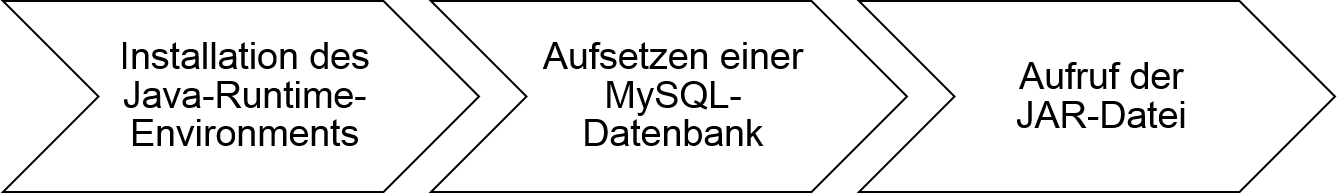
\includegraphics[width=0.8\textwidth]{ErgSoftwareInst1}
	\caption{Schritte der Installation}
	\label{fig:ErgSoftwareInst1}
\end{figure}
Voraussetzung ist das Vorhandensein der aktuellsten Version der Java-Laufzeitumgebung, kurz \textquote{JRE}. Innerhalb der JRE kann die Anwendung betriebssystemunabhängig in der Java-Virtual-Maschine (kurz: \textquote{JVM}) ausgeführt werden. Das Java Runtime Environment ist über die Webseite der Firma ORACLE\footnote{Zum Zeitpunkt der Abgabe des Berichtes ist der Download über folgenden Link möglich: http://www.oracle.com/technetwork/java/javase/downloads/jre8-downloads-2133155.html} zu beziehen und zu installieren.
Weil die Java-Anwendung auf eine MySQL-Datenbank als Persistenzschicht zugreifen soll, wird zusätzlich ein lokaler MySQL-Server benötigt, der über die IP-Adresse 127.0.0.1 / \textquote{localhost} und den Port 3306 erreichbar ist. Das Entwicklerteam empfiehlt den Einsatz des Open-Source-Datenbankservers \textquote{MySQL Community Server}, der ebenfalls von ORACLE\footnote{Zum Zeitpunkt der Abgabe des Berichtes ist der Download über folgenden Link möglich: http://dev.mysql.com/downloads/mysql/} unter der GNU General Public License kostenlos angeboten wird. Ebenfalls empfehlenswert ist die Verwendung des Datenbank-Modellierungs- und Manipulationswerkzeugs \textquote{MySQL Workbench}, das über denselben Weg bezogen werden kann.
Nach der erfolgreichen Installation der beschriebenen Komponenten muss der SQL-Server gestartet werden, um die Datenbank anzulegen. Für Nutzer eines Windows-Betriebssystems sind dazu folgende Schritte erforderlich:

\begin{description}
\item [Starten des MySQL-Server-Dienstes:]
Durch Klick auf \textquote{starten} wird der SQL-Server hochgefahren und der Status ändert sich in \textquote{Gestartet}.
\begin{figure}[ht]
	\centering
	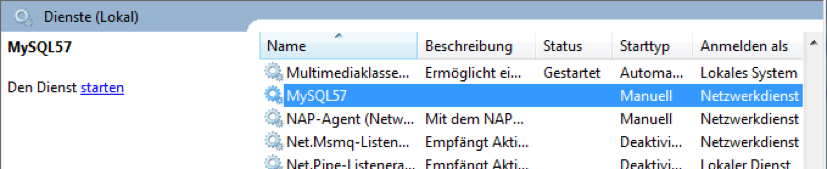
\includegraphics[width=0.8\textwidth]{ErgSoftwareInst2}
	\caption{Starten des MySQL-Server-Dienstes}
	\label{fig:ErgSoftwareInst2}
\end{figure}
\item [Anlegen einer neuen Verbindung zum Server:]
Innerhalb der MySQL-Workbench wird eine Verbindung zum MySQL-Server mit den in Tabelle \ref{tab:mysql} aufgeführten Daten hergestellt.
\begin{table}[ht]
\centering
\caption{Parameter für das Einrichten des DB-Verbindung in der MySQL Workbench}
\label{tab:mysql}
	 \begin{tabular}{cc}
	\textbf{Parameter} & \textbf{Wert}\\
	\hline
	\hline
	Connection Method & Standard (TCP/IP)\\
	 \hline
	Hostname & 127.0.0.1\\
	 \hline
	Port & 3306\\
	 \hline
	Username & NetSimUser\\
	 \hline
	Passwort & NetSimUser\\
	 \end{tabular}
\end{table}
\begin{figure}[ht]
	\centering
	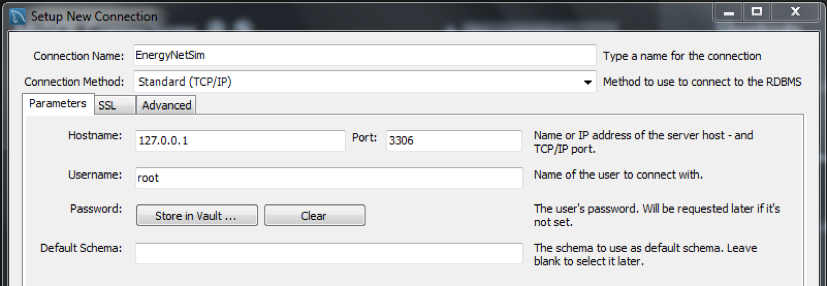
\includegraphics[width=0.8\textwidth]{ErgSoftwareInst3}
	\caption{Konfigurieren einer neuen Verbindung zum MySQL-Server}
	\label{fig:ErgSoftwareInst3}
\end{figure}
\item [Importieren des Datenbank-Schemas:] Das Initialisierungsskript der Datenbank, welches sich im Anhang des Projektberichts befindet, kann daraufhin über Server $ > $ Import Data $ > $ Import from Self-Contained File auf dem neuen MySQL-Server ausgeführt werden. Im Ergebnis existiert nun das Schema \textquote{energynetsimdb}.
\begin{figure}[ht]
	\centering
	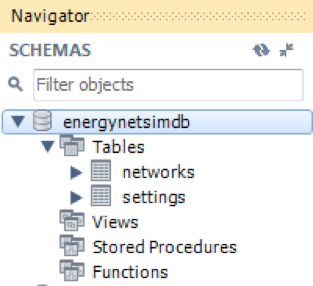
\includegraphics[width=0.4\textwidth]{ErgSoftwareInst4}
	\caption{Das importierte Datenbankschema \textquote{energynetsimdb}}
	\label{fig:ErgSoftwareInst4}
\end{figure}
\item [Ausführen der JAR-Datei:] Durch Doppelklick auf die Datei \textquote{EnergyNetSim.jar} wird das Programm gestartet. Im weiteren Verlauf wird die Verwendung des Programmes aus Endanwender-Sicht geschildert.
\end{description}

\subsubsection{Benutzung der Software zum aktuellem Stand}
Da momentan nur das Rahmenwerk für eine spätere Implementierung von Simulationsansätzen realisiert ist, bietet das Programm nur eine eingeschränkte Funktionalität für den Endnutzer. Auf Erweiterungsmöglichkeiten und dafür vorgesehene Strukturen im Kode wird in Abschnitt \ref{subsubsec:ErgSoftwErweiterung} eingegangen.
\begin{figure}[ht]
	\centering
	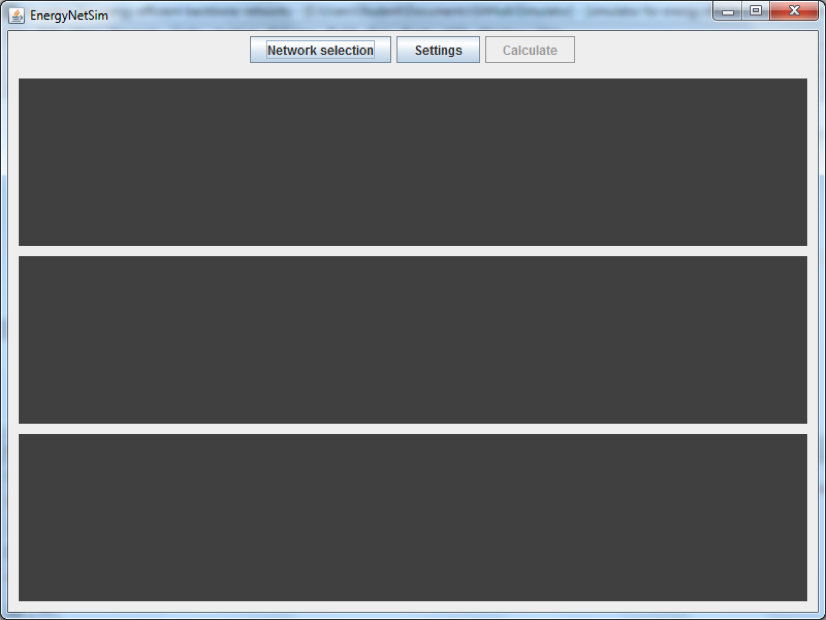
\includegraphics[width=0.6\textwidth]{ErgSoftwareUse1}
	\caption{Hauptfenster nach dem Starten der Software}
	\label{fig:ErgSoftwareUse1}
\end{figure}
Sofern eine Verbindung mit der Datenbank aufgebaut werden konnte, erhält der Benutzer nach Start der Anwendung das Hauptfenster wie in Abbildung \ref{fig:ErgSoftwareUse1} angezeigt. Es besteht die Möglichkeit zur Auswahl verschiedener Netze, die in der Datenbank angelegt wurden, über den Menüpunkt \textquote{Network selection} und zur Änderung von Parametern wie beispielsweise dem Strompreis oder dem Netzlastprofil über die Schaltfläche \textquote{Settings}.
\begin{figure}[ht]
	\centering
	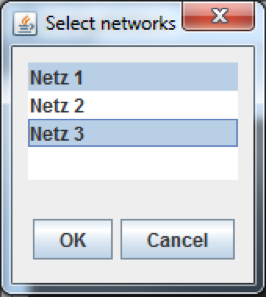
\includegraphics[width=0.2\textwidth]{ErgSoftwareUse2}
	\caption{Dialoge \textquote{Select networks} und \textquote{Settings}}
	\label{fig:ErgSoftwareUse2}
\end{figure}
\begin{figure}[ht]
	\centering
	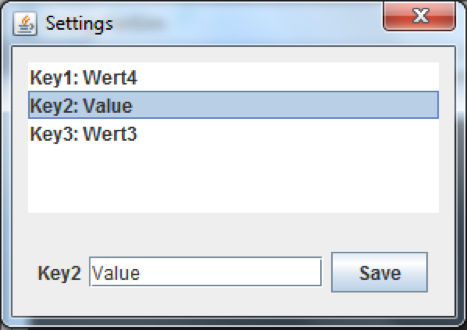
\includegraphics[width=0.4\textwidth]{ErgSoftwareUse3}
	\caption{Dialoge \textquote{Select networks} und \textquote{Settings}}
	\label{fig:ErgSoftwareUse3}
\end{figure}
Die geänderten Werte werden in der Datenbank hinterlegt. In ihr sind statische Ergebniswerte für die Netzlast, den Stromverbrauch und die resultierenden Kosten hinterlegt, deren Ermittlung in Kapitel \ref{subsec:VorgSch} beschrieben wird.
\begin{figure}[ht]
	\centering
	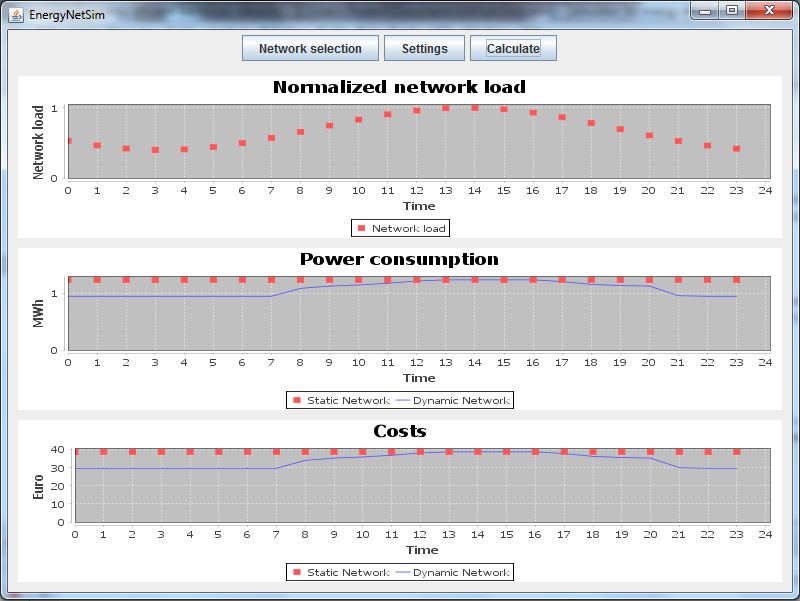
\includegraphics[width=0.8\textwidth]{ErgSoftwareUse4}
	\caption{Ausgabe der Ergebnisse in Diagrammform}
	\label{fig:ErgSoftwareUse4}
\end{figure}
Durch Klick auf die Schaltfläche \textquote{Calculate} werden die Werte in Form von Histogrammen visualisiert.

\subsubsection{Erweiterungsmöglichkeiten} \label{subsubsec:ErgSoftwErweiterung}
Die beschriebene Software stellt keine abgeschlossene Lösung zur Wirtschaftlichkeitsbetrachtung von energieeffizienten Konzepten in simulierten Netzen dar. Wie schon zu Beginn des Kapitels erwähnt, konnte die Entwicklung nicht in der zur Verfügung gestellten Zeit abgeschlossen werden. Vielmehr war die Zielsetzung der Arbeit, eine Anwendung zu erstellen, die es zukünftigen tiefergreifenden Forschungsvorhaben ermöglicht, die fehlenden Algorithmen zu implementieren, welche in Kapitel \ref{subsec:ErgAlg} beschrieben sind, ohne auf Aspekte der grafischen Ausgabe sowie der Anbindung an eine externe Datenbank achten zu müssen.
Das vorliegende Java-Programm erfüllt die gestellten Anforderungen, indem es folgende vordefinierte Methoden und Datenbankstrukturen enthält, die eine Erweiterung um Simulationsalgorithmen zulassen.

\begin{description}
\item [Die Funktion \textquote{calculate()} in der Klasse \textquote{MainModel}.] Bei Klick auf die Schalt\-flä\-che \textquote{Calculate} wird über den Controller in der Klasse \textquote{MainModel} die Funktion \textquote{public void calculate()} aufgerufen. Von dort können der komplette Simulationsalgorithmus gestartet, neue Instanzen von anderen Model-Klassen erzeugt und die erhaltenen Ergebnisse in Form einer Liste gespeichert werden.
\item [Das Package \textquote{models}.] Das Java-Package \textquote{models} bietet Platz für weitere Klassendefinitionen, die von der \textquote{calculate()}-Methode der Klasse \textquote{MainModel} aufgerufen werden und ihrerseits auf die MySQL-Datenbank über die vorhandene Klasse \textquote{DatabaseQueries} zugreifen können. Beispielhaft wurden für die Gerätehardware und die physisch vorhandenen Verbindungen zwischen Knoten die Model-Klassen \textquote{HardwareDevices} und \textquote{Link} angelegt, in denen zukünftig Programmlogik implementiert werden kann.
\item [Das Datenbankschema \textquote{energynetsimdb}.] Im Rahmen des Soft\-ware-Engi\-neering-Pro\-zess\-es wurde ein Datenbankschema entwickelt, das die Datenstruktur für spätere Simulationsalgorithmen abbilden kann. Das zugehörige Enti/-ty-Re\-lation\-ship-Dia\-gramm wurde bereits in Kapitel \ref{subsec:VorgSoftwareEng} vorgestellt und ermöglicht die Generierung der SQL-Create-Befehle für die noch nicht angelegten Relationen.
\end{description}

Zusammenfassend kann festgestellt werden, dass lediglich Änderungen in der Daten- und Logikschicht innerhalb der bereits vorgegebenen Strukturen durchgeführt werden müssen, um den noch nicht kodierten Simulationsalgorithmus einzubinden. Dazu kann der Quellcode im öffentlichen Github-Projekt \textquote{EnergyNetSim/Simulator}\footnote{https://github.com/EnergyNetSim/Simulator} eingesehen und heruntergeladen werden. Es empfiehlt sich, einen eigenen Fork des Projekts zu erzeugen, damit Änderungen ohne großen Aufwand wieder zurück in das Projekt übernommen werden können.


\subsection{Diskussion und Erkenntnisse} \label{subsec:ErgDiskussion}

Zu Beginn der Arbeit setzte sich die Projektgruppe zum Ziel, eine sachlich möglichst richtige Simulation der Netzlast zu entwickeln, um den Energieverbrauch der beiden Netze so realistisch wie möglich abschätzen zu können. 

Schon während der Literaturrecherche war überraschend, dass vorhandene Arbeiten auf dem Gebiet sich immer mit einem kleinen Untergebiet des Themas beschäftigen -- Ein Standardwerk zum Stand der Forschung unter Kombination aller vorhandenen Technologien existiert nicht. Das beweist, dass die Forschungen zu energieeffizienten Netztechnologien noch kein abgeschlossenes Gebiet beschreiben.

Sobald mit der Entwicklung des Algorithmus angefangen wurde, stellte sich heraus, dass für ein valides Ergebnis die Simulation sehr komplex werden musste. Hierbei stellten sich folgende Herausforderungen:
\begin{itemize}
	\item In den Nodes sind jeweils Geräte verschiedener Layer nötig, um das weitere Routing zu gewährleisten. 
	\item Für eine realistische Berechnung der Netzlast reicht eine stundenweise Iteration nicht aus. Pro Stunde würde von jeder Quelle ein konstanter Datenstrom ausgehen, was in der Realität so nicht der Fall ist.
	\item Die Einhaltung der QoS Parameter konnt mit dem gewählten Ansatz nicht ge\-währ\-lei\-stet werden.
	\item Die Kompatibilität der Konzepte zur Erhöhung der Energieeffizienz konnte nicht abschließend geklärt werden.
\end{itemize}

Um eine Umsetzung des Algorithmus zu ermöglichen, mussten also sehr viele Annahmen getroffen werden. Hierdurch geht das eigentliche Ziel, eine sachlich richtige Simulation durchzuführen, weitgehend verloren, da im Vergleich zu echten existierenden Backbone-Netzwerken die Vergleichbarkeit und damit die Praxistauglichkeit der Simulation nicht gegeben ist.

Stattdessen wurde ein solides Grundgerüst in Softwareform entwickelt, auf das weitere Forschungen aufsetzen können. Es erleichtert die Implementierung von Algorithmen wie jenen, die im Kapitel 4 beschrieben wurden, da die Konzeption in dieser Arbeit bereits umfänglich beschrieben wird. Zur Darstellung der Potenziale von energieeinsparenden Verfahren wurde auf vorhandene Forschungsergebnisse aufgesetzt.

Bei Betrachtung des Gesamtverbrauchs resultiert ein Energieeinsparpotenzial von 23,5 Prozent pro Jahr  \cite[5]{Chiaraviglio2009}, in Geldeinheiten\cite{Proteus2016} bewertet, 91.500 Euro. Die Modellierung des Netzes orientierte sich an \cite{Chiaraviglio2009}, worin ein Netz ähnlich dem eines großen italienischen Carriers definiert wird. Skaliert man das Einsparpotenzial auf einen großen europäischen Telekommunikationskonzern wie die Deutsche Telekom AG, ergeben sich weit größere Summen, die gespart werden können. Hierbei ist zu beachten, dass weitere Einsparungen durch die Integration zusätzlicher energiesparender Technologien wie Hybrid Optical Switching erreicht werden können.